\documentclass{ximera}

\usepackage{epsfig}

\graphicspath{
  {./}
  {figures/}
}


\usepackage{morewrites}

%\newcounter{ccounter}
%\setcounter{ccounter}{1}
%\newcommand{\Chapter}[1]{\setcounter{chapter}{\arabic{ccounter}}\chapter{#1}\addtocounter{ccounter}{1}}

%\newcommand{\section}[1]{\section{#1}\setcounter{thm}{0}\setcounter{equation}{0}}

%\renewcommand{\theequation}{\arabic{chapter}.\arabic{section}.\arabic{equation}}
%\renewcommand{\thefigure}{\arabic{chapter}.\arabic{figure}}
%\renewcommand{\thetable}{\arabic{chapter}.\arabic{table}}

%\newcommand{\Sec}[2]{\section{#1}\markright{\arabic{ccounter}.\arabic{section}.#2}\setcounter{equation}{0}\setcounter{thm}{0}\setcounter{figure}{0}}

\newcommand{\Sec}[2]{\section{#1}}

\setcounter{secnumdepth}{2}
%\setcounter{secnumdepth}{1} 

%\newcounter{THM}
%\renewcommand{\theTHM}{\arabic{chapter}.\arabic{section}}

\newcommand{\trademark}{{R\!\!\!\!\!\bigcirc}}
%\newtheorem{exercise}{}

\newcommand{\dfield}{{\sf dfield9}}
\newcommand{\pplane}{{\sf pplane9}}

\newcommand{\EXER}{\section*{Exercises}}%\vspace*{0.2in}\hrule\small\setcounter{exercise}{0}}
\newcommand{\CEXER}{}%\vspace{0.08in}\begin{center}Computer Exercises\end{center}}
\newcommand{\TEXER}{} %\vspace{0.08in}\begin{center}Hand Exercises\end{center}}
\newcommand{\AEXER}{} %\vspace{0.08in}\begin{center}Hand Exercises\end{center}}

% BADBAD: \newcommand{\Bbb}{\bf}

\newcommand{\R}{\mbox{$\Bbb{R}$}}
\newcommand{\C}{\mbox{$\Bbb{C}$}}
\newcommand{\Z}{\mbox{$\Bbb{Z}$}}
\newcommand{\N}{\mbox{$\Bbb{N}$}}
\newcommand{\D}{\mbox{{\bf D}}}
\usepackage{amssymb}
%\newcommand{\qed}{\hfill\mbox{\raggedright$\square$} \vspace{1ex}}
%\newcommand{\proof}{\noindent {\bf Proof:} \hspace{0.1in}}

\newcommand{\setmin}{\;\mbox{--}\;}
\newcommand{\Matlab}{{M\small{AT\-LAB}} }
\newcommand{\Matlabp}{{M\small{AT\-LAB}}}
\newcommand{\computer}{\Matlab Instructions}
\newcommand{\half}{\mbox{$\frac{1}{2}$}}
\newcommand{\compose}{\raisebox{.15ex}{\mbox{{\scriptsize$\circ$}}}}
\newcommand{\AND}{\quad\mbox{and}\quad}
\newcommand{\vect}[2]{\left(\begin{array}{c} #1_1 \\ \vdots \\
 #1_{#2}\end{array}\right)}
\newcommand{\mattwo}[4]{\left(\begin{array}{rr} #1 & #2\\ #3
&#4\end{array}\right)}
\newcommand{\mattwoc}[4]{\left(\begin{array}{cc} #1 & #2\\ #3
&#4\end{array}\right)}
\newcommand{\vectwo}[2]{\left(\begin{array}{r} #1 \\ #2\end{array}\right)}
\newcommand{\vectwoc}[2]{\left(\begin{array}{c} #1 \\ #2\end{array}\right)}



\newcommand{\inv}{^{-1}}
\newcommand{\CC}{{\cal C}}
\newcommand{\CCone}{\CC^1}
\newcommand{\Span}{{\rm span}}
\newcommand{\rank}{{\rm rank}}
\newcommand{\trace}{{\rm tr}}
\newcommand{\RE}{{\rm Re}}
\newcommand{\IM}{{\rm Im}}
\newcommand{\nulls}{{\rm null\;space}}

\newcommand{\dps}{\displaystyle}
\newcommand{\arraystart}{\renewcommand{\arraystretch}{1.8}}
\newcommand{\arrayfinish}{\renewcommand{\arraystretch}{1.2}}
\newcommand{\Start}[1]{\vspace{0.08in}\noindent {\bf Section~\ref{#1}}}
\newcommand{\exer}[1]{\noindent {\bf \ref{#1}}}
\newcommand{\ans}{}
\newcommand{\matthree}[9]{\left(\begin{array}{rrr} #1 & #2 & #3 \\ #4 & #5 & #6
\\ #7 & #8 & #9\end{array}\right)}
\newcommand{\cvectwo}[2]{\left(\begin{array}{c} #1 \\ #2\end{array}\right)}
\newcommand{\cmatthree}[9]{\left(\begin{array}{ccc} #1 & #2 & #3 \\ #4 & #5 &
#6 \\ #7 & #8 & #9\end{array}\right)}
\newcommand{\vecthree}[3]{\left(\begin{array}{r} #1 \\ #2 \\
#3\end{array}\right)}
\newcommand{\cvecthree}[3]{\left(\begin{array}{c} #1 \\ #2 \\
#3\end{array}\right)}
\newcommand{\cmattwo}[4]{\left(\begin{array}{cc} #1 & #2\\ #3
&#4\end{array}\right)}

\newcommand{\Matrix}[1]{\ensuremath{\left(\begin{array}{rrrrrrrrrrrrrrrrrr} #1 \end{array}\right)}}

\newcommand{\Matrixc}[1]{\ensuremath{\left(\begin{array}{cccccccccccc} #1 \end{array}\right)}}



\renewcommand{\labelenumi}{\theenumi)}
\newenvironment{enumeratea}%
{\begingroup
 \renewcommand{\theenumi}{\alph{enumi}}
 \renewcommand{\labelenumi}{(\theenumi)}
 \begin{enumerate}}
 {\end{enumerate}\endgroup}



\newcounter{help}
\renewcommand{\thehelp}{\thesection.\arabic{equation}}

%\newenvironment{equation*}%
%{\renewcommand\endequation{\eqno (\theequation)* $$}%
%   \begin{equation}}%
%   {\end{equation}\renewcommand\endequation{\eqno \@eqnnum
%$$\global\@ignoretrue}}

%\input{psfig.tex}

\author{Martin Golubitsky and Michael Dellnitz}

%\newenvironment{matlabEquation}%
%{\renewcommand\endequation{\eqno (\theequation*) $$}%
%   \begin{equation}}%
%   {\end{equation}\renewcommand\endequation{\eqno \@eqnnum
% $$\global\@ignoretrue}}

\newcommand{\soln}{\textbf{Solution:} }
\newcommand{\exercap}[1]{\centerline{Figure~\ref{#1}}}
\newcommand{\exercaptwo}[1]{\centerline{Figure~\ref{#1}a\hspace{2.1in}
Figure~\ref{#1}b}}
\newcommand{\exercapthree}[1]{\centerline{Figure~\ref{#1}a\hspace{1.2in}
Figure~\ref{#1}b\hspace{1.2in}Figure~\ref{#1}c}}
\newcommand{\para}{\hspace{0.4in}}

\renewenvironment{solution}{\suppress}{\endsuppress}

\ifxake
\newenvironment{matlabEquation}{\begin{equation}}{\end{equation}}
\else
\newenvironment{matlabEquation}%
{\let\oldtheequation\theequation\renewcommand{\theequation}{\oldtheequation*}\begin{equation}}%
  {\end{equation}\let\theequation\oldtheequation}
\fi

\makeatother


\title{Least Squares Approximations}

\begin{document}
\begin{abstract}
\end{abstract}
\maketitle

  \label{S:LSA}

Let $W\subset\R^n$ be a subspace and $x_0\in\R^n$ be a vector.  In this
section we solve a basic geometric problem and investigate some of its
consequences.  The problem is:
\begin{quote}
Find the vector $w_0\in W$ that is the nearest vector in $W$ to $x_0$.
\end{quote}

\begin{definition} \rm \label{D:least_squares}
The vector $w_0$ in the subspace $W$ of $\R^n$ that is the nearest to the 
vector $x_0$ in $\R^n$ is called the \em{least squares approximation} of 
$x_0$ in $W$.
\end{definition} 

\begin{figure}[htb]
        \centerline{%
        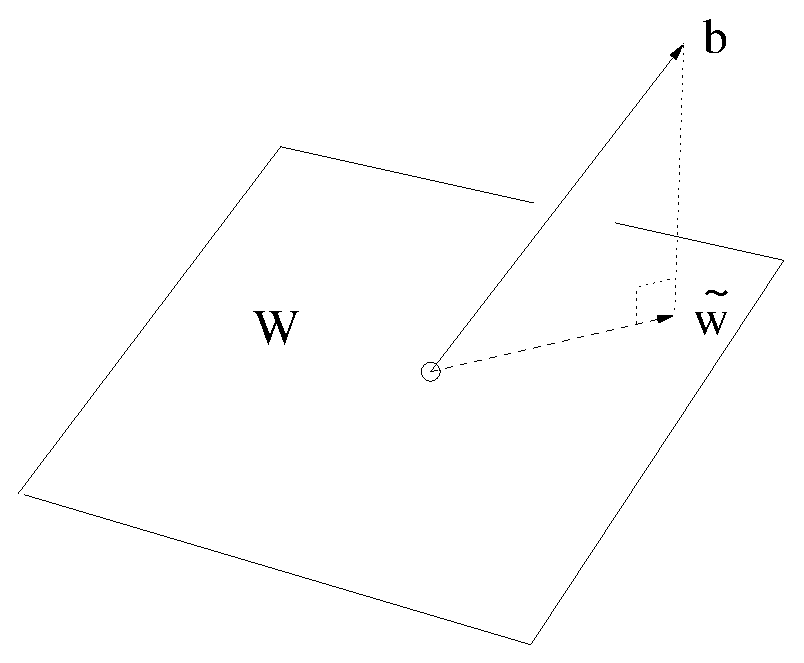
\psfig{file=../figures/nearest.eps,width=2.5in}}
        \caption{The vector $w_0$ is the least squares approximation of the vector $x_0$ by a vector in $W$.}
        \label{F:nearest}
\end{figure}


The distance between two vectors\index{distance!between vectors}
$v$ and $w$ is $||v-w||$.  Hence the least squares approximation 
can be rephrased as follows: find a vector $w_0\in W$ such that
\begin{equation}  \label{E:leastsq}
||x_0-w_0||\leq ||x_0-w|| \quad \forall w\in W.
\end{equation}
Condition \eqref{E:leastsq} is also called the
{\em least squares approximation}\index{least squares!approximation}.
In order to see where this name comes from we write \eqref{E:leastsq} in the
equivalent form
\begin{equation} \label{E:LS_inequality}
||x_0-w_0||^2\leq ||x_0-w||^2 \quad \forall w\in W.
\end{equation}
The form \eqref{E:LS_inequality} means that the sum of the squares of the
components of the vectors $x_0 - w$ is minimal at $w = w_0$.

Before continuing, we state and prove 
\begin{lemma}[The Law of Pythagorus] \index{Law of Pythagorus}  \label{L:LP}
The vectors $z_1,z_2\in\R^n$ are orthogonal if and only if  
\begin{equation} \label{E:LP}
||z_1+z_2||^2 = ||z_1||^2 + ||z_2||^2.
\end{equation}
\end{lemma}

\begin{proof}
To verify \eqref{E:LP} calculate 
\begin{align*}
  ||z_1+z_2||^2&=(z_1+z_2)\cdot(z_1+z_2) \\
  &=z_1\cdot z_1 +2z_1\cdot z_2+z_2\cdot z_2 \\
  &=||z_1||^2 + 2z_1\cdot z_2 +||z_2||^2.
\end{align*}
It follows that $z_1$ and $z_2$ satisfy \eqref{E:LP} if and only if $z_1\cdot z_2 = 0$  
if and only $z_1$ and $z_2$ are orthogonal.
\end{proof}

Using \eqref{E:leastsq} and \eqref{E:LP}, we can rephrase the minimum distance 
problem as follows.
\begin{lemma}  \label{L:orthoLSA}
The vector $w_0\in W$ is the closest vector to $x_0\in\R^n$ if the vector 
$x_0-w_0$ is orthogonal to every vector in $W$. (See Figure~\ref{F:nearest}.)
\end{lemma}

\begin{proof}  Write $x_0-w=z_1+z_2$ where $z_1=x_0-w_0$ and $z_2=w_0-w$.  By 
assumption, $x_0-w_0$ is orthogonal to every vector in $W$; so $z_1$ and 
$z_2\in W$ are orthogonal.  It follows from \eqref{E:LP} that
\[
||x_0-w||^2 = ||x_0-w_0||^2 + ||w_0-w||^2.
\]
Since $||w_0-w||^2\ge 0$, \eqref{E:leastsq} is valid, and $w_0$ is the vector 
nearest to $x_0$ in $W$. \end{proof}

\subsubsection*{Least Squares Distance to a Line}
\index{least squares!distance to a line}
\index{distance!to a line}

Suppose $W$ is as simple a subspace as possible; that is, suppose $W$ is one
dimensional with basis vector $w$.  Since $W$ is one dimensional, a vector
$w_0\in W$ that is closest to $x_0$ must be a multiple of $w$; that is,
$w_0=aw$.  Suppose that we can find a scalar $a$ so that $x_0-aw$ is
orthogonal to every vector in $W$.  Then it follows from
Lemma~\ref{L:orthoLSA} that $w_0$ is the closest vector in $W$ to $x_0$.
To find $a$, calculate
\[
0 = (x_0-aw)\cdot w = x_0\cdot w - a w\cdot w.
\]
Then
\[
a = \frac{x_0\cdot w}{||w||^2}
\]
and
\begin{equation}  \label{E:singleortho}
w_0 = \frac{x_0\cdot w}{||w||^2} w.
\end{equation}
Observe that $||w||^2\not=0$ since $w$ is a basis vector.

For example, if $x_0=(1,2,-1,3)\in\R^4$ and $w=(0,1,2,3)$.  The the vector
$w_0$ in the space spanned by $w$ that is nearest to $x_0$ is
\[
w_0 = \frac{9}{14}w
\]
since $x_0\cdot w=9$ and $||w||^2=14$.

\subsubsection*{Least Squares Distance to a Subspace}
\index{least squares!distance to a subspace}
\index{distance!to a subspace}

Similarly, using Lemma~\ref{L:orthoLSA} we can solve the general least
squares problem by solving a system of linear equations.  Let
$w_1,\ldots,w_k$ be a basis for $W$ and suppose that
\[
w_0 = \alpha_1w_1 + \cdots + \alpha_kw_k
\]
for some scalars $\alpha_i$.  We now show how to find these scalars.

\begin{theorem}  \label{T:nearestvector}
Let $x_0\in\R^n$ be a vector and let $\{w_1,\ldots,w_k\}$ be a
basis\index{basis} for the subspace\index{subspace} $W\subset\R^n$.
Then
\begin{equation} \label{e:w_0_in_basis}
w_0 = \alpha_1w_1 + \cdots + \alpha_kw_k
\end{equation}
is the nearest vector in $W$ to $x_0$ when
\begin{equation}  \label{E:nearestvector}
\left(\begin{array}{c} \alpha_1 \\ \vdots \\ \alpha_k \end{array}\right) =
(A^tA)\inv A^tx_0,
\end{equation}
where $A=(w_1|\cdots|w_k)$ is the $n\times k$ matrix whose columns are the
basis vectors of $W$.
\end{theorem}

\begin{proof} Observe that the vector $x_0-w_0$ is orthogonal to every vector in $W$
precisely when $x_0-w_0$ is orthogonal to each basis vector $w_j$.  It
follows from Lemma~\ref{L:orthoLSA} that $w_0$ is the closest vector to $x_0$
in $W$ if
\[
(x_0-w_0)\cdot w_j = 0
\]
for every $j$.  That is, if
\[
w_0\cdot w_j = x_0\cdot w_j
\]
for every $j$.  These equations can be rewritten as a system of equations in
terms of the $\alpha_i$, as follows:
\begin{equation}  \label{E:dots}
 \begin{array}{ccc}
w_1\cdot w_1\alpha_1 + \cdots + w_1\cdot w_k\alpha_k & = & w_1\cdot x_0\\
 & \vdots &  \\
w_k\cdot w_1\alpha_1 + \cdots + w_k\cdot w_k\alpha_k & = & w_k\cdot x_0.
\end{array}
\end{equation}

Note that if $u,v\in\R^n$ are column vectors, then $u\cdot v= u^tv$. Therefore,
we can rewrite \eqref{E:dots} as
\[
A^tA \left(\begin{array}{c} \alpha_1\\ \vdots \\ \alpha_k \end{array}\right) =
A^tx_0,
\]
where $A$ is the matrix whose columns are the $w_j$ and $x_0$ is viewed as a
column vector.  Note that the matrix $A^tA$ is a $k\times k$ matrix.

We claim that $A^tA$ is invertible.  To verify this claim, it suffices to
show that the null space\index{null space}
of $A^tA$ is zero; that is, if $A^tA z = 0$ for some
$z\in\R^k$, then $z=0$.  First, calculate
\[
||Az||^2 = Az\cdot Az = (Az)^tAz = z^tA^tAz= z^t0 = 0.
\]
It follows that $Az=0$.  Now if we let $z=(z_1,\ldots,z_k)^t$, then the
equation $Az=0$ may be rewritten as
\[
z_1w_1 + \cdots + z_kw_k = 0.
\]
Since the $w_j$ are linearly independent, it follows that the $z_j=0$.  In
particular, $z=0$.  Since $A^tA$ is invertible, \eqref{E:nearestvector} is
valid, and the theorem is proved. 
\end{proof}

\begin{corollary} \label{C:nearestvector}
Let $x_0$ be a vector in $\R^n$, let $W$ be a subspace of $\R^n$, and
let $w_1,\ldots,w_k$ in $\R^n$ be a basis for $W$.
Let $A = (w_1|\cdots| w_k)$ be an $n\times k$ matrix.  Then 
\begin{equation} \label{C:w_0_formula}
w_0 =  A(A^tA)\inv A^tx_0.
\end{equation}
 is the least squares approximation to $x_0$ in $W$.
\end{corollary}

\begin{proof}
Define scalars $\alpha_1,\ldots,\alpha_k$ by \eqref{E:nearestvector}.  It follows 
from Theorem~\ref{T:nearestvector} that the least squares approximation is
\[ 
w_0 = A \left(\begin{array}{c} \alpha_1 \\ \vdots \\ \alpha_k \end{array}\right) = A(A^tA)\inv A^tx_0, 
\]
as claimed.
\end{proof}

\includeexercises

\end{document}

%%% Local Variables:
%%% mode: latex
%%% TeX-master: "../linearAlgebra"
%%% End:
